\documentclass{article}
%%%%%%%%%%%%%%%%%%%%%%%%%%%%%%%%%%%%%%%%%%%%%%%%%%%%%%%%%%%%%
% Lecture Specific Information to Fill Out
%%%%%%%%%%%%%%%%%%%%%%%%%%%%%%%%%%%%%%%%%%%%%%%%%%%%%%%%%%%%%
\newcommand{\LectureTitle}{L21: Volume Rendering}
%\newcommand{\LectureDate}{\today}
\newcommand{\LectureDate}{March 27, 2015}
\newcommand{\LectureClassName}{CS 557}
\newcommand{\LatexerName}{Peter Henderson}
%%%%%%%%%%%%%%%%%%%%%%%%%%%%%%%%%%%%%%%%%%%%%%%%%%%%%%%%%%%%%

% Change "article" to "report" to get rid of page number on title page
\usepackage{amsmath,amsfonts,amsthm,amssymb}
\usepackage{setspace}
\usepackage{Tabbing}
\usepackage{fancyhdr}
\usepackage{lastpage}
\usepackage{extramarks}
\usepackage{chngpage}
\usepackage{soul,color}
\usepackage{graphicx,float,wrapfig}
\usepackage{afterpage}
\usepackage{abstract}
\usepackage{pgfplots}
\usepackage{caption}
\usepackage{listings}
\usepackage{url}

% In case you need to adjust margins:
\topmargin=-0.45in
\evensidemargin=0in
\oddsidemargin=0in
\textwidth=6.5in
\textheight=9.0in
\headsep=0.25in
\tikzstyle{cnstyle}=[domain=0:1, samples=100, ultra thick]

% Setup the header and footer
\pagestyle{fancy}
\lhead{\LatexerName}
\chead{\LectureClassName: \LectureTitle}
\rhead{\LectureDate}
\lfoot{\lastxmark}
\cfoot{}
\rfoot{Page\ \thepage\ of\ \pageref{LastPage}}
\renewcommand\headrulewidth{0.4pt}
\renewcommand\footrulewidth{0.4pt}

%%%%%%%%%%%%%%%%%%%%%%%%%%%%%%%%%%%%%%%%%%%%%%%%%%%%%%%%%%%%%
% Some tools
\newcommand{\enterTopicHeader}[1]{\nobreak\extramarks{#1}{#1 continued on next page\ldots}\nobreak
                                    \nobreak\extramarks{#1 (continued)}{#1 continued on next page\ldots}\nobreak}
\newcommand{\exitTopicHeader}[1]{\nobreak\extramarks{#1 (continued)}{#1 continued on next page\ldots}\nobreak
                                   \nobreak\extramarks{#1}{}\nobreak}

\newlength{\labelLength}
\newcommand{\labelAnswer}[2]
  {\settowidth{\labelLength}{#1}
   \addtolength{\labelLength}{0.25in}
   \changetext{}{-\labelLength}{}{}{}
   \noindent\fbox{\begin{minipage}[c]{\columnwidth}#2\end{minipage}}
   \marginpar{\fbox{#1}}

   % We put the blank space above in order to make sure this
   % \marginpar gets correctly placed.
   \changetext{}{+\labelLength}{}{}{}}

\setcounter{secnumdepth}{0}
\newcommand{\TopicName}{}
\newcounter{TopicCounter}
\newenvironment{Topic}[1][Problem \arabic{TopicCounter}]
  {\stepcounter{TopicCounter}
   \renewcommand{\TopicName}{#1}
   \section{\TopicName}
   \enterTopicHeader{\TopicName}}
  {\exitTopicHeader{\TopicName}}

\setcounter{secnumdepth}{0}
\newcommand{\ExampleSectionName}{}
\newcounter{ExampleSectionCounter}[TopicCounter]
\newenvironment{ExampleSection}[1][Example \arabic{ExampleSectionCounter}]
  {\stepcounter{ExampleSectionCounter}
   \renewcommand{\ExampleSectionName}{#1}
   \section{\ExampleSectionName}
   \enterTopicHeader{\ExampleSectionName}}
  {\exitTopicHeader{\ExampleSectionName}}

\setcounter{secnumdepth}{0}
\newcounter{ExampleBoxCounter}[TopicCounter]
\newcommand{\examplebox}[1]
  {
  % We put this space here to make sure we're disconnected from the previous
   % passage
   \stepcounter{ExampleBoxCounter}
   \noindent\fbox{\begin{minipage}[c]{\columnwidth}#1\end{minipage}}\enterTopicHeader{\ExampleSectionName}\exitTopicHeader{\ExampleSectionName}\marginpar{\fbox{\#\arabic{ExampleBoxCounter}}}
   % We put the blank space above in order to make sure this
   % \marginpar gets correctly placed.
   \vskip10pt
   }

\renewcommand{\contentsname}{{\normalsize Topics Covered}}
\renewcommand{\abstractname}{\LectureTitle\ Summary}
\renewcommand{\absnamepos}{flushleft}

\pgfplotsset{vasymptote/.style={
    before end axis/.append code={
        \draw[densely dashed] ({rel axis cs:0,0} -| {axis cs:#1,0})
        -- ({rel axis cs:0,1} -| {axis cs:#1,0});
    }
}}

%%%%%%%%%%%%%%%%%%%%%%%%%%%%%%%%%%%%%%%%%%%%%%%%%%%%%%%%%%%%%

\begin{document}
\begin{spacing}{1.1}
\newpage

% When topics are long, it may be desirable to put a \newpage or a
% \clearpage before each Topic environment
%\newpage
\begin{Topic}[Volume Rendering \Roman{TopicCounter}]
Clouds, fire smoke, fog, etc. are difficult to model with vertices and polygons. Visualization of 3d point data is also difficult such as medical imaging. hence volume rendering comes in.
\subsection{How to display scalar field (i.e. 3D data like MRI)?}
The kinds of images we're thinking about here are MRI scans or 3D renderings of point data. Two general approaches:
\begin{itemize}
\item integrating density along rays to the camera
\item displaying level surfaces ("iso-surfaces")
\end{itemize}
The questions we're trying to answer in terms of CS are: How to select surfaces from 3D data and render them? What are the costs?
\subsection{Integrating density along rays}
You have 3D data divided into $N \times \text{2D images}$, assume each layer is an RGBA image. Given two semi-transparent layers we can blend pixels as follows.

With two layers we can use the following:
\begin{itemize}
\item Assume $F, B$ are foreground and background pixels from two layers.
\item Let $(r,g,b \alpha) = (\alpha R, \alpha G, \alpha B, \alpha)$ Blend pixels as follows
\begin{itemize}
\item $FB_{rgb\alpha} = F_{rgb\alpha} + (1 - F_{\alpha}) B_{rgb\alpha}$
\item Basically, you add a scaled version of the background opacity according to the clear part of $\alpha$
\end{itemize}
\end{itemize}

With N layers, we can use the 2 layer system recursively. We can then see that the $\alpha$ for a layer $k$ will be equal to:
$$\alpha_k (1 - \alpha_1) (1 - \alpha_2) \dots (1 - \alpha_{k-1}) = \alpha_k \Pi_{j=1}^{k-1} (1 - \alpha_j)$$
This can be thought of as you are taking the clear portion of all the preceding layers ($1-\alpha_i$) and using up whatever opaque ($\alpha_k$) part of your layer you have. Thus, the \textbf{accumulated opacity} of N layers is:

$$ \sum_{k=1}^{N} \alpha_k \Pi_{j=1}^{k-1} (1 - \alpha_j)$$

Then, the RGB image of the N layers ($L_i$) is a weighted sum of the N, RGB images.

$$ (L_1 \circ L_2 \circ \dots \circ \L_N)_{rgb} = \sum_{k=1}^{N} (R_k, G_k, B_k) \alpha_k \Pi_{j=1}^{k-1} (1 - \alpha_j)$$

\begin{ExampleSection}
So what's an example of this in action? OpenGL fog! OpenGL 1.x provides a special case that we have uniform fog + opaque rendered surface. So then given a fog depth between 0 and 1. OpenGl does the following:


\begin{center}
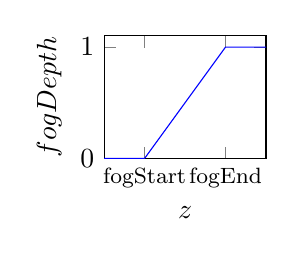
\begin{tikzpicture}
  \begin{axis}[width=.3\columnwidth,xlabel={$z$},ylabel={$fogDepth$},xmin=0,xmax=4,ymin=0,
ymax=1.1,xtick=\empty, ytick=\empty, xtick={1, 3 ,4}, xticklabels={\footnotesize  $\text{fogStart}$, \footnotesize$\text{fogEnd}$, }, ytick={0,1}, yticklabels={$0$,$1$},    samples=1000]]  %yshift=0.7ex,
\addplot[blue]{(x>=1 && x <= 3)*(-.5 + .5*x) + (x>3)};
  \end{axis}
\end{tikzpicture}
\includegraphics[scale=0.25]{images/fog_graphs}
\end{center}

$$ I_{rgb} = I_{RGB} \alpha^{fog} + I_{RGB}^{fog} (1-\alpha^{fog})$$

Where $I_{rgb}$ is the rendered value of the visible surface (e.g. Blinn-Phong). $ I_{RGB}^{fog}$ is the color of the fog. $\alpha^{fog}$ depends on the fog depth. The three formulas the OpenGL uses for calculating this $\alpha^{fog}$ value are (as seen in graph):

\[
\alpha^{fog} = \left\{
     \begin{array}{lr}
       1-fogDepth & : \# fogMode = GL_LINEAR\\
       e^{-fogDepth*GL\_FOG\_DENSITY} & : \# fogMode = GL\_EXP\\
       e^{(-fogDepth*GL\_FOG\_DENSITY)^2} & : \# fogMode = GL\_EXP2
     \end{array}
   \right.
   \]

And the different OPENGL fog settings are:
\begin{lstlisting}{c}
glFogfv(GL_FOG_COLOR, fogColor); //I^fog_RGB
glFogf(GL_FOG_DENSITY, .35); // How dense will the fog be?
glFogf(GL_FOG_START, 1); //where does fogStart
glFogf(GL_FOG_END, 2); //where does fogEnd
glEnable(GL_FOG);
glFogi(GL_FOG_MODE, fogMode);
\end{lstlisting}

But how did they derive these formulas? Well let's take the GL\_EXP formula.

We use $1-\alpha_j \approx e^{-\alpha_j}$ as we assume $\alpha_j$ is small for all j and $\alpha_0 = 0$.

So, then we know:

$$\Pi_{j=0}^{k-1} (1-\alpha_j) = \Pi_{j=0}^{k-1} e^{-\alpha_j} = e^{-\sum_{j=1}^{k-1} \alpha_j}$$

Now, if we assume uniform fog density such that:

$$\alpha_j = \alpha, \forall j > 0$$

Then,

$$\Pi_{j=1}^{k-1} (1-\alpha_j) = e^{-(k-1)\alpha}$$

Thus, if the fog color $I_{RGB}^{fog}$ is also constant then the contribution of the fog alone is:
$$\alpha I_{RGB}^{fog} \sum_{k=1}^{N} e^{-(k-1)\alpha} $$
$$= \alpha I_{RGB}^{fog} \frac{1-e^{-N\alpha}}{1-e^{-\alpha}}$$.

Since, $1-e^{-\alpha} \approx \alpha$ and $e^{-N\alpha} = e^{-fogDepth*GL\_FOG\_DENSITY} = \alpha^{fog}$ we get that

$$ I^{fog}_{rgb} = I_{RGB}^{fog}(1-\alpha^{fog})$$

and thus

$$I_{rgb} = I_{RGB} \alpha^{fog} + I_{RGB}^{fog} (1-\alpha^{fog})$$.


\end{ExampleSection}

\subsection{Where do the RGBA values come from?}

\begin{itemize}
\item emission/absorption (assume the material is emitting light)
\item texture mapping (paint a function onto the objects)
\item rendering with light and material (e.g. Blinn-Phong)
\end{itemize}

\subsubsection{Emission/Absorption Model}
When discussing Blinn-Phong model in OpenGL, we said that RGB color of surfaces was the sum of three components: DIFFUSE, SPECULAR, AMBIENT. However, there is also a GL\_EMISSION component. This component is independent of any lighting. It is added to the other three components.

\textit{Normally if one uses Blinn-Phong then one doesn't include an emission component and similarly if one uses an emission component then one doesn't include the other three components.}

\textit{For blending N layers, one could be to use an emission component for the RGB colors. The alpha would account for ``absorption''.}

\subsubsection{3D Texture Mapping}

Consider a 3D scalar texture or a 3D RGBA texture. The texture coordinates for indexing into the RGBA values are (s, t, p, q). This allows us to perform perspective mappings -- i.e. a class of deformations -- on the textures. Similar idea as homographies but 4D, so more general. You can think of the 3D coordinates as (s, t, p, 1).

You can now define texture coordinates on the corners of a cube. If you define a planar slice through the cube, OpenGL will interpolate the texture coordinates for you. Plane slices are sometimes referred to as \textbf{proxy geometry}. So basically you're viewing slices of the texture instead of the entire volume and that's where you get your RGB values from, the slices.
\\\\
\textbf{Tri-Linear Interpolation}

\begin{center}
\includegraphics[scale=0.25]{images/trilinear_interp}
\end{center}

The intersection of a ray with the plane slices will not occur exactly at the grid points where the data is defined.

\subsection{Transfer Function}
In many applications such as in medical imaging, we have scalar data values (not RGBA) defined over a 3D volume e.g. cube. Usually the data values are normalized to [0, 1]. We need to define a \textbf{transfer function} which maps data values to RGBA values. Essentially it is a ``lookup table''. A transfer function can be represented as a 1D texture, i.e. it maps data values in [0, 1] to RGBA values. Basically, you're saying you want to transfer some data value (i.e. the MRI scan data, etc.) and map it to some RGBA values. \textit{Note transfer function domain says nothing about position.}

There is no right way to define a transfer function for a given 3D data set. It is an interactive process.\footnote{Can see the following for an example at around 1:30... \url{https://www.youtube.com/watch?v=dmh-8nKSzTc}} So you take your data cube values according to a distribution and map a histogram. You can use this a guide to try and differentiate different materials based on spikes. Choose control points and set opacity (classification) and RGB (shading), and interpolate.

\subsection{How do we render level surfaces? (iso-surfaces)}

Levoy et al. (1988)\footnote{\url{https://graphics.stanford.edu/papers/volume-cga88/}} is able to show the air-skin, skin-bone interface from MRI scans.

We don't want to compute polygonal representations of these surfaces (geometric primitives). Rather, we assign surface normals to all the points within the volume and then compute the RGB color using Blinn-Phong or some other model. Thus, we need to define a surface normal and a material at each point in the volume (plus a lighting model). The material can be defined by a transfer function. Define a surface normal at (x,y,z) by the 3D gradient of data value f(x,y,z).

$$ \nabla f(x,y,z) = ((f(x+1, y, z) - f(x-1, y, z))/2, (f(x, y+1, z) - f(x, y-1, z))/2, (f(x, y, z+1) - f(x, y, z-1))/2)$$
$$n(x, y, z) = \frac{\nabla f(x,y,z)}{\|\nabla f(x,y,z)\|}$$

The boundary between two regions A and B with data values a and b, respectively, is characterized by a large gradient and by data values in some range. So for example, within the skin or within the air thickness the data will be constant, but between the two there is a gradient significantly greater than 0. To render the boundary region between A and B, define the opacity component of the transfer function using both the data f(x,y,z) and its gradient. In a transition region (i.e. high gradient region) has a high opacity ($\alpha = 1$) and everywhere else is transparent.\footnote{For details, see Kniss, Joe, et al. ``Gaussian transfer functions for multi-field volume visualization.'' Visualization, 2003.}

Many transfer functions were invented in decade between ~1995 and ~2005. There is still no consensus on what is a good transfer function. Many dependencies:

\begin{itemize}
\item What is the user's goal?
\item How class/instance specific should it be?
\item How much work is required by user to define it?
\end{itemize}

No best solution, but many possible ones.

\end{Topic}

\end{spacing}
\end{document}